
\section{Visualization}
\label{sec:visualization}

% Describe each visual components briefly
Our visualization tool as shown in Figure~\ref{fig:teaser} satisfies not only the basic visual design requirements, but also the motivated specific requirements mentioned in Section~\ref{sec:design}.
The tool consists of the following components:
\begin{itemize}
\item \textit{Training Accuracy Graph:} This standard line graph (Figure~\ref{fig:teaser} (A)) shows the accuracy changes of train and validation sets according to each epoch (R1).
\item \textit{Classification View:} The classification view (Figure~\ref{fig:teaser} (F)) visualizes each categorized samples according to the predicted classes and the calculated predicted scores for a selected epoch (R1).
\item \textit{Predicted Probability Distribution View:} This parallel coordinate visualization (Figure~\ref{fig:teaser} (E)) reveals the predicted score distributions over classes of selected samples by users (R2).
\item \textit{Detail View:} Our detail view  (Figure~\ref{fig:teaser} (D)) shows sample's features learned by neural networks, for example important sentences and words (R3).
\end{itemize}
The following subsections describe these components in detail.

\begin{figure}[tb]
\centering
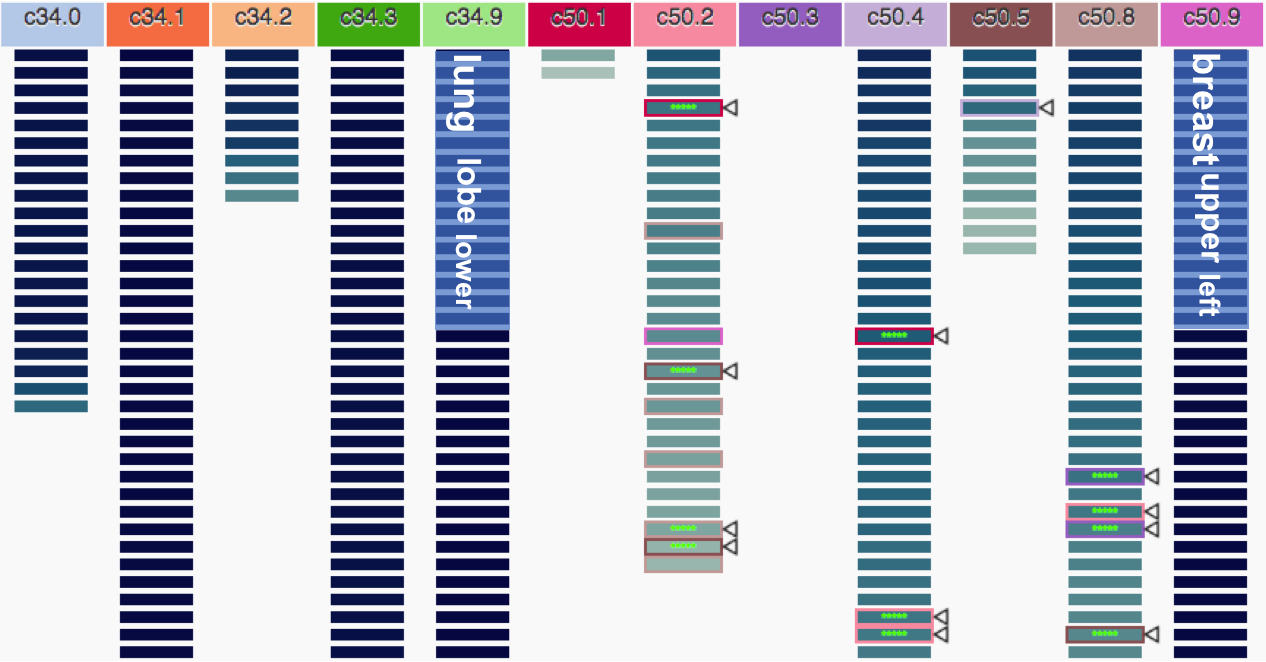
\includegraphics[width=1.0\columnwidth]{classification-view_v2}
\caption{Classification View: Samples (small narrow boxes) are visualized according to their predicted classes. The box colors represent their predicted scores. Outlined boxes are incorrectly predicted samples.
Small triangles denote the samples whose the misclassified number is more than mis-prediction threshold value.}
\label{fig:classification-view}
%\vspace{-0.8cm}
\end{figure}

\subsection{Classification View}
Our classification view is to explore classification results and to identify misclassified samples.
For each sample, neural networks usually produce predicted scores across all classes.
The class with the highest score is selected as the predicted class.
The columns in the view (Figure~\ref{fig:classification-view}) represent the classes and each column head has its class name and an unique color.
Under the heads, each narrow box corresponds a sample (a pathology report in this paper) and the boxes are lined along their predicted class columns and ordered by their scores.
For each class, the stacked boxes as a whole is a bar that is a suitable visual variable for comparing quantity (the number of samples for each class)~\cite{cleveland1984graphical}. 
A sample is selected by users, we add green markers inside the box.
Once users change the epoch using the slider control (Figure~\ref{fig:teaser} (B)) and then the classification view dynamically updates the result corresponding to the current selected epoch.

The solid boxes for each column represent samples correctly predicted while the outlined boxes represent samples incorrectly predicted.
The fill color of each box indicates the predicted score assigned to the predicted class.
The score is varied from 0 to 1 and the sum of the scores is 1.
%since the score set for a sample is a softmax output.
In other words, the boxes with the dark blue color are predicted with high confidence while the boxes with the light blue color are predicted with low confidence.
This allows to inspect the samples that are ambiguously classified\textemdash its predicted scores are evenly distributed across all classes.
In addition, the color gradient of stacked boxes as a whole shows that how confidently the model classifies the samples for the corresponding class.
It possibly suggests the directions to increase the accuracy of the model.
The outline color of a misclassified sample indicates the class which the sample is labeled as.
The misclassified samples usually have relatively low confidence as shown in Figure~\ref{fig:classification-view}.
Also, we provide a different type of visualization for the classification view as an alternative option as shown in Figure~\ref{fig:grid-mode}.
This type can handle more number of samples and is useful when we use a small size of display.

If the number of incorrect prediction for a sample is greater than the value of the mis-prediction threshold slider (Figure~\ref{fig:teaser} (C)) as epochs progress, we indicate the samples with the small triangles.
This allows to see that what samples are continuously mis-predicted during the training process.
Users can examine the samples using the detail view to find reasons for misclassification.

Also, we extract a set of words considered to be important by HAN from samples for each class and allow to display those over the column by user selection (This function is not completely implemented yet).
The font size of each word indicates its importance.
For example, we display a set of three keywords for each of the two selected columns: \textit{c34.9} and \textit{c50.9} as shown in Figure~\ref{fig:classification-view}.
We can see what are the major keywords of each class even though we have no background knowledge on the reports and classes.

\subsection{Predicted Probability Distribution View}
Our visual analytics system utilizes a standard parallel coordinate visualization to enable examining of the predicted score distributions over classes for the selected samples.
As we mentioned previously, to increase the classification accuracy, it is important to know what samples are incorrectly predicted and how their predicted scores are distributed.
%, and what classes are secondly or thirdly predicted.
We show an example case in Figure~\ref{fig:prodis}.
We select the samples that are predicted as a class (c50.4) with low confidence (Figure~\ref{fig:prodis} (A)).
The numbers of incorrect prediction of the selected samples are greater than the mis-prediction threshold value set as 10.
We can see their predicted score distributions as shown in Figure~\ref{fig:prodis} (B).
We filter the samples whose scores assigned to another class (c50.8) are over 0.3 as shown in Figure~\ref{fig:prodis} (C).
We can see that the model confuses the two classes, \textit{c50.4} and \textit{c50.8}.
This can provide an opportunity to investigate why the model cannot clearly distinguish between the two different classes.

\begin{figure}[tb]
\centering
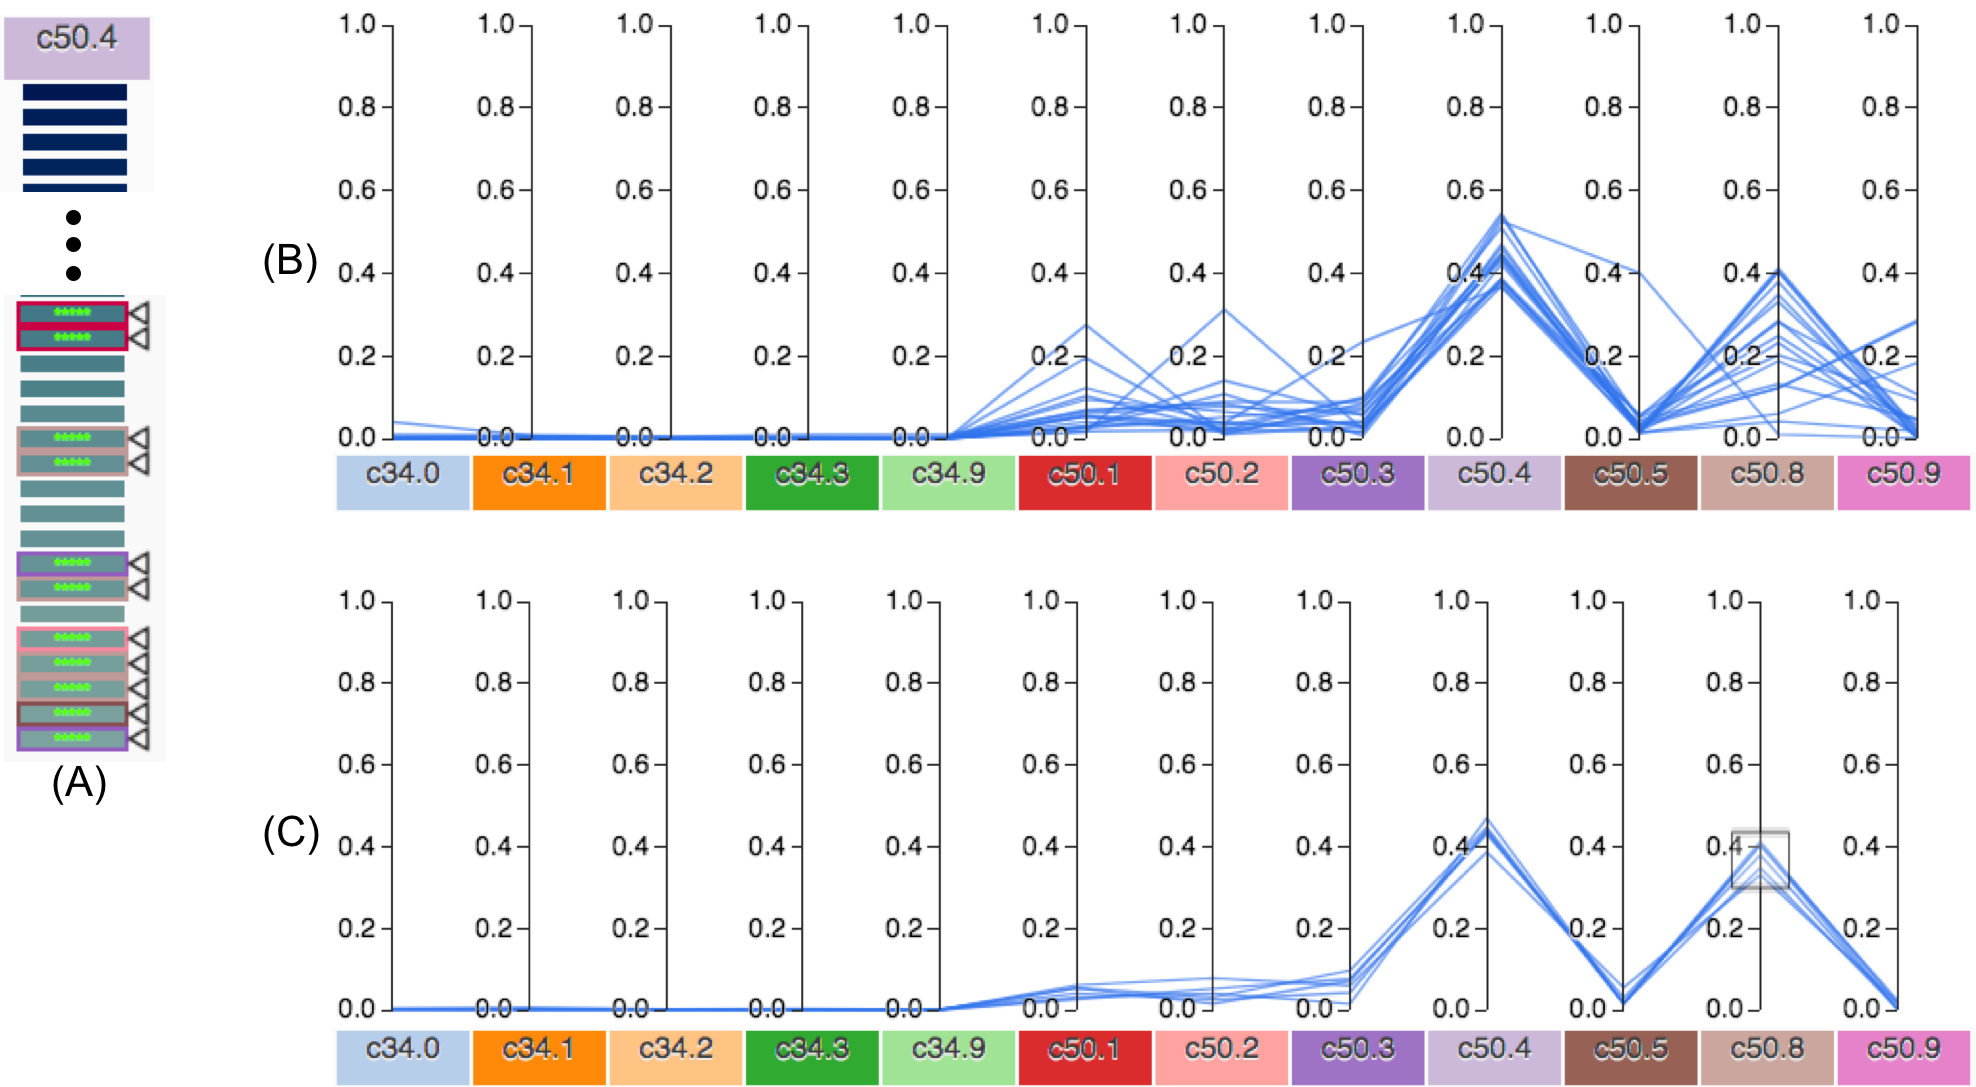
\includegraphics[width=1.0\columnwidth]{prodis_v2}
\caption{Selected samples in the class, c50.4 (A). The predicted score distributions of the selected samples (B). Filtering the samples with its score of the class, c50.8 over 0.3 (C). The model confuses the two classes: c50.4 and c50.8}
\label{fig:prodis}
%\vspace{-0.8cm}
\end{figure}

\subsection{Detail View}
Finally, our detail view visualizes the features of each sample learned by the neural networks.
An example is shown in Figure~\ref{fig:detail-view}.
We utilize the Hierarchical Attention Network (HAN) described in Section~\ref{sec:background} to extract important words and sentences from a huge volume of pathology reports and to classify the reports.
For each report, we visualize the words and the lines (sentences) with their importance in the detail view.
The dark red and dark blue colors denote highly important lines and words, respectively.
On the other hand, the light blue and red colors denote little important lines and words.
In the example view in Figure~\ref{fig:detail-view}, we can see the highlighted important words and lines which usually include the important words.
In this paper the detail view supports only a document type of data, but it is possible to visualize the learned features of other types of data.
For example, in image classification, we can highlight the learned features on an image using other feature detection techniques~\cite{zhou2016learning}.
We leave this as a future work.
















